%++++++++++++++++++++++++++++++++++++++++
% Don't modify this section unless you know what you're doing!
\documentclass[letterpaper,12pt]{article}
\usepackage[utf8]{inputenc}
\usepackage{float}
\usepackage{tabularx} % extra features for tabular environment
\usepackage{amsmath}  % improve math presentation
\usepackage{graphicx} % takes care of graphic including machinery
\usepackage[margin=1in,letterpaper]{geometry} % decreases margins
\usepackage{cite} % takes care of citations
\usepackage[final]{hyperref} % adds hyper links inside the generated pdf file
\usepackage[table,xcdraw]{xcolor}
\hypersetup{
	colorlinks=true,       % false: boxed links; true: colored links
	linkcolor=blue,        % color of internal links
	citecolor=blue,        % color of links to bibliography
	filecolor=magenta,     % color of file links
	urlcolor=blue         
}
%++++++++++++++++++++++++++++++++++++++++


\begin{document}

\title{Práctica 3 - Ruteo}
\author{Matthew Aguerreberry, Natasha Tomattis}
\date{\today}
\maketitle

% \begin{abstract} 
% \end{abstract}


\section{Practica de Ruteo - OSPF}
\begin{figure}[ht] 
        
	\centering 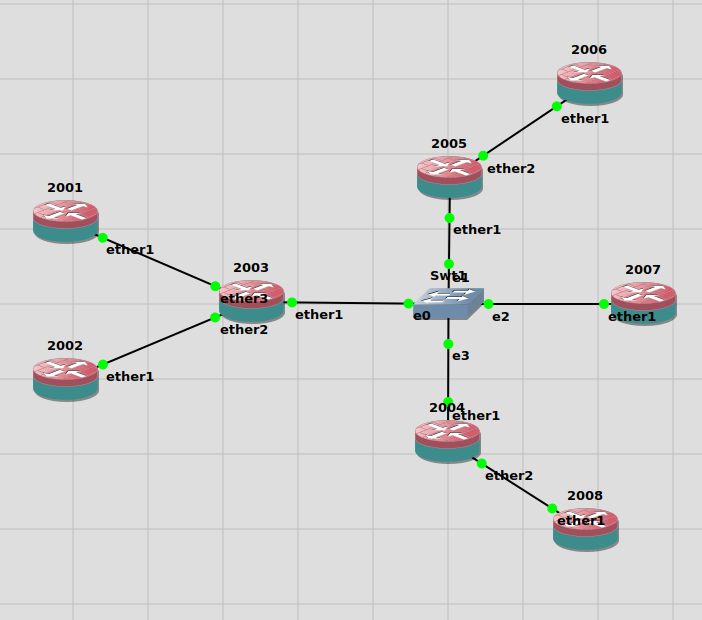
\includegraphics[width=0.8\columnwidth]{figure/topo_figura1.png}
	%\includegraphics[width=1.0\columnwidth]{sr_setup.pdf}
	\caption{
			\label{fig:samplesetup} % spaces are big no-no 
			Implementación Ejercicio 1.
	}
\end{figure}
	\begin{enumerate}
		\item \textbf{Conectar los routers, switchs y nodos segun el diagrama de la figura 1}
		\item \textbf{Congurar las interfaces de acuerdo al diagrama}
		\item \textbf{Congurar OSPF en todas los routers respetando las areas segun el diagrama. Es posible alcanzar todas las redes?}\\
		Si, todas las redes son compartidas a traves de OSPF
		\item \textbf{Los routers de las areas no backbone, conocen todas las rutas a las demas redes?}\\
		Si, la division de areas no limita la propagacion de rutas OSPF.
		\item \textbf{Observando el area backbone, que router fue elegido como DR y cual como BDR? Por que fueron elegidos esos routers?}\\
		\item 
	\subsection{Enlaces consultados}
	\end{enumerate}
	\begin{itemize}
		\item{HCNA Networking Study Guide}  \\
		\textit{Springer. Huawei Technologies Co., Ltd.},Ch 8.2 RIP.
		\item{Temporizadores de RIP}  \\
		\url{http://www.redescisco.net/sitio/2010/07/19/temporizadores-de-rip/}
	\end{itemize}
\end{document}